\section{Scomposizione del requisito}

Per semplicità divido il requisito in diversi punti e per ognuno ne spiego la soluzione
o metodologia utilizzata:

\begin{enumerate}
    \item\label{animationenum:1} Le animazioni devono essere disponibili in qualunque sezione o vista in cui si trovi l'utente e definite dal contesto attuale;

    \item\label{animationenum:2} Ogni CardView deve essere trascinabile dall'utente;
    
    \item\label{animationenum:3} Nel momento in cui l'utente usa una forza di trascinamento superiore a un valore di soglia tutte le viste devono
        cadere per gravità;

    \item\label{animationenum:4} Ogni CardView mostrerà un contenuto dinamico differente e definito da dei componenti
    limitati specifici;

    \item\label{animationenum:5} Le animazioni in questione devono essere progettate in pagine, in cui ogni pagina può contenere 
    più CardView. L'utente vedrà in un determinato momento una e soltanto una pagina. 
    Una volta che le CardView acquisisco una gravità e cadono, finirà l'animazione o apparirà
    una nuova pagina, se presente;

    \item\label{animationenum:7} Ogni CardView deve interagire con le altre della stessa pagina, come se si toccassero;

\end{enumerate}

% % % % % % % % % % % % % % % % % % % % % % % % % % % % % % % % % % % % %
%                      Onnipresenza delle animazioni                    %
% % % % % % % % % % % % % % % % % % % % % % % % % % % % % % % % % % % % %
\subsection{Presentazione delle animazioni}

Per creare animazioni definite dal contesto usiamo quindi un semplice UIViewController che gestirà tutte le animazioni,
ma invece di presentarlo attraverso i metodi base visti alla sezione~\ref{sec:navigation}, lo presentiamo al di sopra della \textbf{UIWindow} (vedere sezione~\ref{sec:uiwindow}),
in modo da non essere vincolati dal contesto dell'utente quando l'animazione finirà, ma allo stesso tempo
consentire il controllo dell'inizializzazione del UIViewController in base al contesto attuale.

\subsection{Aggiunta del ViewController nella UIWindow}

L'animazione viene inizializzata nel ViewController, in questo caso \textbf{mainViewController},
genitore di tutto il contesto, in modo da avere il controllo su tutto 
il contesto. Questo perchè tutti i ViewController nello stack di navigazione possono
essere chiusi a seguito di un qualunque evento dell'animazione, avendo così un controllo molto accuranto
del contenuto che l'utente visualizzerà alla fine dell'animazione.

\begin{minted}{swift}
let keyWindow: UIWindow?

if #available(iOS 13.0, *) {
    keyWindow = UIApplication.shared.connectedScenes
    .filter({$0.activationState == .foregroundActive})
    .map({$0 as? UIWindowScene})
    .compactMap({$0})
    .first?.windows
    .filter({$0.isKeyWindow}).first
} else {
    keyWindow = UIApplication.shared.keyWindow
}

mainViewController.addChild(currentAnimationViewController!)

// Aggiungiamo la vista del nostro viewController alla UIWindow
keyWindow?.addSubview(currentAnimationViewController!.view)

// Mostriamo il viewController
currentAnimationViewController!.didMove(toParent: mainViewController)
\end{minted}

% % % % % % % % % % % % % % % % % % % % % % % % % % % % % % % % % % % % %
%                        CardView trascinabile                          %
% % % % % % % % % % % % % % % % % % % % % % % % % % % % % % % % % % % % %
\subsection{Aggiunta di una gesture}\label{gestureimplemention}

Per un'animazione che ha necessità di muoversi come se l'utente la stesse spostando trascinando sullo schermo occore una \textbf{UIPanGestureRecognizer}.
Dalla documentazione delle UIGestureRecognizer viene spiegato che ogni vista "draggabile" necessita una  e solo una gesture,
per questo ogni card view dovrà averne una diversa. Di seguito il codice di implementazione

\begin{minted}{swift}
// Durante il settaggio delle cardview
// aggiungo la vista alla parentView
parentView.addSubview(view)

// Creo la gesture
let panGesture = UIPanGestureRecognizer(target: target, action: action)

// Assegno un nome che verrà utilizzato come lock
// per impedire la concorrenza di due gesture differenti
panGesture.name = "gesture-\(index)"

// Aggiungo la gesture alla cardView
cardView.addGestureRecognizer(panGesture)
\end{minted}

I parametri target e action sono rispettivamente il viewController che gestisce la gesture e il metodo
che deve essere eseguito quando avviene una PanGesture.
Di seguito l'implementazione del metodo handlePan che gestisce tutte le gesture di una stessa pagina.

\begin{minted}{swift}
private let activeGesture = nil

// Metodo chiamato dalla UIPanGesture
@objc private func handlePan(_ recognizer:
    UIPanGestureRecognizer) {

    // Lock per evitare che due gesture
    // funzionino in contemporanea
    if let gestureName = activeGesture,
        recognizer.name != gestureName {
        return
    } else {
        activeGesture = recognizer.name
    }
    
    // CardView che viene mossa dall'utente
    let animatedView = recognizer.view!
    
    // Coordinate del punto di tocco
    // rispetto alla vista principale
    let touchInView = recognizer.location(in: self.view)

    // Coordinate del punto di
    // tocco rispetto alla cardView
    let touchInAlert = recognizer.location(in: animatedView)
    let velocity = recognizer.velocity(in: self.view)
    
    // Ottengo l'offset rispetto al centro della cardView
    let offset = UIOffset(
        horizontal: touchInAlert.x - animatedView.bounds.midX,
        vertical: touchInAlert.y - animatedView.bounds.midY
    )

    // Aggingo i comportamenti iniziali
    self.createPageDynamicBehaviours()
    self.addCheckForDismiss()
    
    // Attivo e disattivo i comportamenti del UIDynamicAnimator
    // in base agli stati delle PanGesture
    switch recognizer.state {
    case .began:
        self.configureForStartDragging(animatedView,
            with: offset,
            touchPointInView: touchInView,
            touchPointInAlert: touchInAlert
        )
    case .changed:
        // Sposto la cardView attraverso un attachmentBehavior
        dragAttachmentBehavior.anchorPoint = touchInView
    case .cancelled, .ended, .failed:
        self.configureForFinishDragging(animatedView,
            with: velocity,
            offset: offset
        )
        // Disattivo il lock
        activeGesture = nil
    default:
        break
    }
}
\end{minted}

% % % % % % % % % % % % % % % % % % % % % % % % % % % % % % % % % % % % %
%                        Gravity                                     %
% % % % % % % % % % % % % % % % % % % % % % % % % % % % % % % % % % % % %
\subsection{Aggiunta della gravità }

Attraveso la UIPanGesture è possibile calcolare il vettore della velocità del trascinamento.
Con questo semplice dato e ciò che abbiamo studiato dello UIKit Dynamics è possibile aggiungere una gravità solo se
il vettore della velocità è superiore a una soglia prestabilita.

Per implementarlo è stato utilizzato un UIGravityBehavior, inizializzato in questo modo:

\begin{minted}{swift}
    let gravityBehavior = UIGravityBehavior(items: page.views)
    gravityBehavior.magnitude = Constants.gravity
\end{minted}

Il valore \textbf{magnitude} è la forza di gravità che vogliamo
assegnare alle viste in questione. \\

Nella figura~\ref{fig:6} si vede lo schermo di uno smartphone, che presenta l'animazione
voluta in questo caso con due CardView. Ognuna di esse ha un \textbf{UIAttachmentBehavior} al
centro per fare in modo che sia sempre centrata in esso (o nel punto di drag dell'utente),
un \textbf{UICollisionBehavior} per permettere che durante il drag le CardView possa scontrarsi e non si accavallino e un \textbf{UIGravityBehavior}, il quale 
viene utilizzato per la caduta delle viste alla fine dell'animazione o al cambiamento di pagina.

In più esiste uno speciale UIAttachmentBehavior tra i centri delle due CardView per permettere che il movimento di una
sposti anche l'altra, è una sorta di corda che le lega.

Per l'ingresso invece è stato inserito un UISnapBehavior, al centro per ogni oggetto, che anima 
gli oggetti dando un effetto a molla.

Tutte le animazioni sono attivate e disattivate in specifici momenti, questo dipende 
dalla UIPanGestureRecognizer e dai movimenti dell'utente.

% % % % % % % % % % % % % % % % % % % % % % % % % % % % % % % % % % % % %
%                        Modular CardView                               %
% % % % % % % % % % % % % % % % % % % % % % % % % % % % % % % % % % % % %
\subsection{La CardView modulare}

L'intero UIViewController che regola le CardView animate è stato progettato per presentare 
animazioni con contenuti dinamici, per questo sono state progettate delle strutture dati specifiche per consentire la personalizzazione
del contenuto di ogni CardView. 

Inizialmente sono stati definiti i possibili componenti che ogni CardView può adottare:
\begin{itemize}
    \item\textbf{Solo testo}: Il componente include un testo, il suo colore e il colore di sfondo.
    \item\textbf{Solo Immagine}: Il componente include un'immagine e il colore di sfondo.
    \item\textbf{Row}: Il componente include un'icona e due testi in quest'ordine.
    \item\textbf{Animazione Lottie\cite{lottie}}: Il componente include una semplice UIView in cui viene mostrata un'animazione Lottie.
    \item\textbf{Footer}: Il componente include del testo e un'icona sulla destra.
\end{itemize}

Una volta definiti tutti i componenti per ogni CardView questa viene assemblata "incollando" un componente
dopo l'altro attraveso una vista chiamata ModularCardView. In figura~\ref{fig:7}, si può vedere un esempio del risultato finale ottenuto. \\

\begin{minipage}{\linewidth}
    \centering
    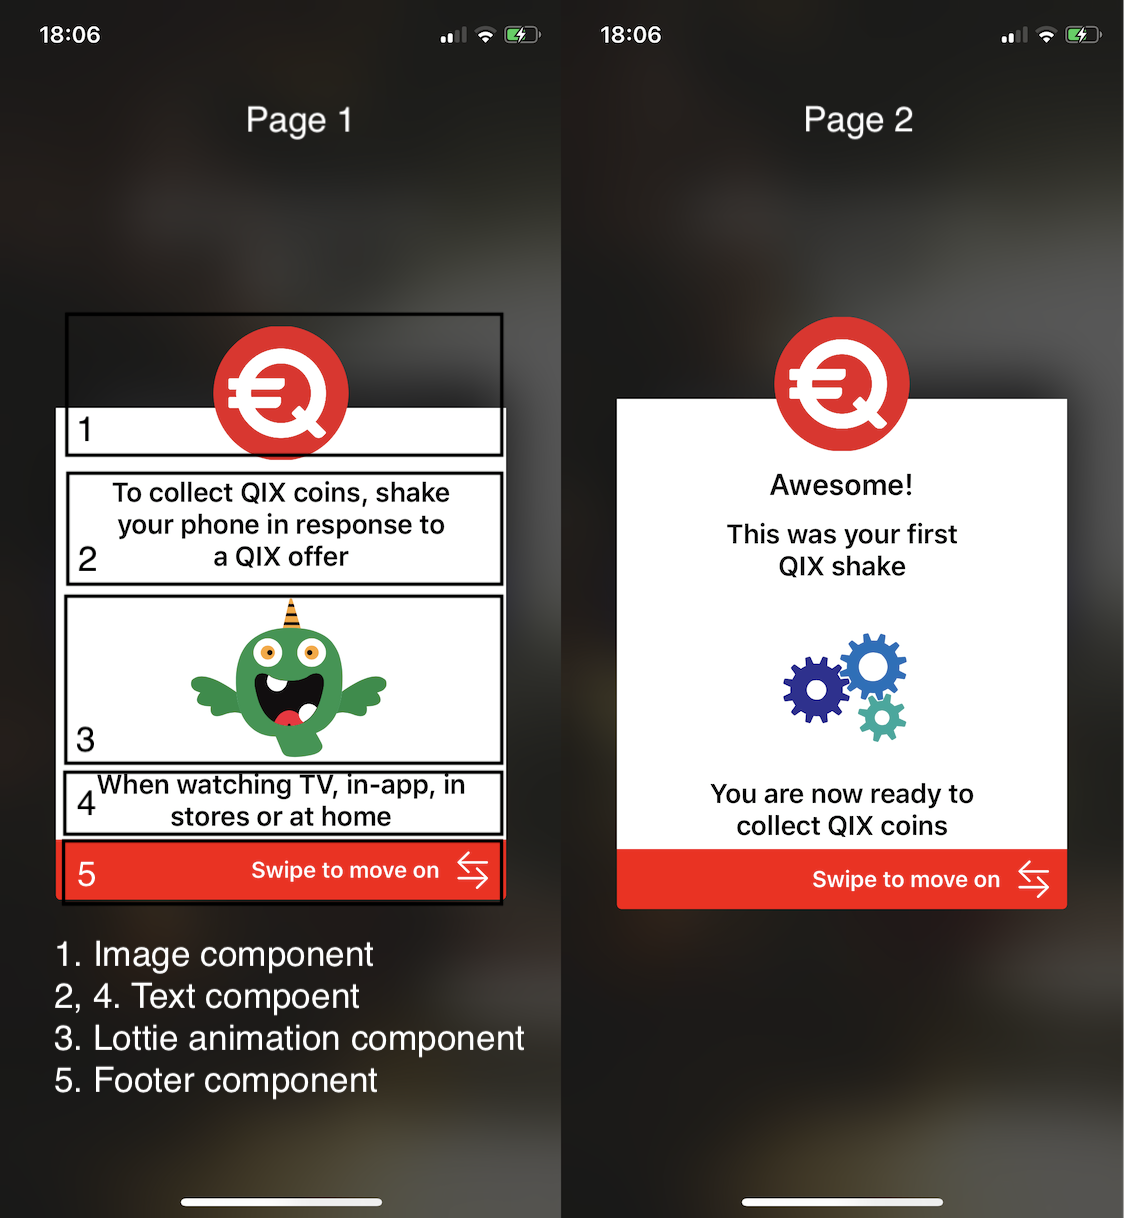
\includegraphics[width=10cm]{an12}
    \captionof{figure}{
       CardViews modulari
    }
    \label{fig:7}
\end{minipage}\\

Dopo aver creato ogni componente separatamente ho creato la \textbf{ModularCardView}.
Questa vista attraverso un array di UIView, ossia i componenti, utilizza dei constraints 
per assemblarli insieme. Vediamo di seguito il metodo \textbf{build}:

\begin{minted}{swift}
// Creo un array di constraints
var constraints = [NSLayoutConstraint]()
    
// Creo un loop enumerato sull'array dei componenti
for (index, view) in components.enumerated() {
    // Disabilito l'autoresizing mask automatico
    view.translatesAutoresizingMaskIntoConstraints = false
    
    // Aggiugo il componente alla ModulaCardView
    self.addSubview(view)
    
    // Aggiungi i constraint a destra e sinistra
    constraints.append(contentsOf: [
        view.leadingAnchor.constraint(equalTo: 
            self.leadingAnchor),
        view.trailingAnchor.constraint(equalTo:
            self.trailingAnchor)
    ])
    
    if components.count > 1 {

        if index == 0 {
            // Al primo componente setto il top
            // della ModulaView
            constraints.append(
                view.topAnchor.constraint(equalTo:
                    self.topAnchor)
            )
        } else {
            // Ai sucessivi setto top anchor il bottom
            // anchor dell'elemento precedente
            let bottomAnchor = 
                components[index - 1].bottomAnchor
            constraints.append(
                view.topAnchor.constraint(equalTo:
                    bottomAnchor)
            )
        }
        
        // Se è l'ultimo componente gli aggiugo un constraint
        // alla fine della ModularView
        if index == components.count - 1 {
            constraints.append(
                view.bottomAnchor.constraint(equalTo:
                    self.bottomAnchor)
            )
        }
    } else {
        // Esiste un solo componente,
        // gli setto i constraint sopra e sotto
        constraints.append(contentsOf: [
            view.topAnchor.constraint(equalTo:
                self.topAnchor),
            view.bottomAnchor.constraint(equalTo:
                self.bottomAnchor)
        ])
    }
}

// Attivo tutti i constraints
NSLayoutConstraint.activate(constraints)
\end{minted}

% % % % % % % % % % % % % % % % % % % % % % % % % % % % % % % % % % % % %
%                   La paginazione delle animazioni                     %
% % % % % % % % % % % % % % % % % % % % % % % % % % % % % % % % % % % % %
\subsection{Paginazione delle animazioni}

Avendo definito al punto uno l'utilizzo di un solo UIViewController per le animazioni da un lato viene semplificata
la presentazione delle stesse, dato che basterà presentare un solo UIViewController, ma dall'altro verrà delegata
l'intera paginazione al view controller. \\

In particolare questo UIViewController accetta come variabile di inizializzazione
un array di pagine e in base allo stato della UIPanGestureRecognizer deciderà se passare alla pagina successiva
o interrompere l'animazione.

% % % % % % % % % % % % % % % % % % % % % % % % % % % % % % % % % % % % %
%                   La paginazione delle animazioni                     %
% % % % % % % % % % % % % % % % % % % % % % % % % % % % % % % % % % % % %
\subsection{Il Collider}

Come accennato al punto~\ref{animationenum:3} le CardView hanno dei comportamenti fisici definiti
da UIKit Dynamics. In particolare, per conferire un effetto di collisione viene usato un \textbf{UICollisionBehavior} e implementato come segue:

\begin{minted}{swift}
    let itemsCollisionBehavior = UICollisionBehavior(items:
        page.views)
\end{minted}

In questo modo ogni oggetto con questo
comportamento riuscirà a scontrarsi con gli altri oggetti simili.
